\documentclass[11pt]{ctexart}

\usepackage{multicol}
%\usepackage{mwe}
\usepackage{subfigure}
\usepackage{mathtools}
\usepackage{graphicx}
\usepackage{amsmath}
\usepackage{mathrsfs}
\usepackage[top=0.5in,bottom=1in,left=1in,right=1in]{geometry}
\usepackage{pdflscape}
\usepackage{times}
\usepackage{bm}
%\usepackage{setspace}
\usepackage{color}
\usepackage{caption}
\usepackage{amsmath}
\usepackage{amssymb}
\usepackage{CJK}
\usepackage{longtable}
%\usepackage[final]{pdfpages}
\usepackage{listings}
\usepackage{textcomp}
\usepackage{xcolor}
\usepackage{algorithm2e}
\usepackage{float}
\usepackage{algorithmicx}
\usepackage{algpseudocode}
\usepackage{hyperref}

\hypersetup{hidelinks,
	colorlinks=true,
	allcolors=black,
	pdfstartview=Fit,
	breaklinks=true}

\pagestyle{plain}




\begin{document}

\title{第十二周实习报告20220613}
\author{宋欣源}
\date{\today}

\maketitle % need full-width title

\CTEXsetup[format={\Large\bfseries}]{section}

\section{第一,综述}

下面对于这些天实习的工作做一个报告。现在就这一周的工作做一个总结
我这周主要在raw3数据集上进行。首先是继续上次新的backbone骨架的研究,然后基于CNN2d进行了研究,最后尝试着提高模型稳定性

\section{第二,CNN1d}
这段时间的CNN1d没有像上面的结果一样从层的堆叠和意义以及信息流的角度进行设计,而是从CNN1d的角度重新开始卷积层和特征提取。不再基于某个backbone而是进行自己的研究。

\subsection{模型和表现}

基于上一周的经验,发现尺缩模型稳定性较差,尺度缩窄以后,后面的模型提取的信息具有更大的不确定性,不能很好的表现所有数据的特性,那么还是采取最后加入avgpool的方式提高模型在时间序列的表现。

模型1:普通CNN1d(CNN1d(5,1)*3+relu+CNN1d(3,1)+

CNN1d(1,1)*2+relu+linear)

模型表现{\kaishu \small IC: 0.053, pnl:2.55}

~\\
模型2:普通CNN1d(CNN1d(5,1)*3+relu+avg+CNN1d(3,1)+

CNN1d(1,1)*2+avg+relu+linear)

模型表现{\kaishu \small IC: 0.059, pnl:2.578}


~\\
模型3:普通CNN1d(CNN1d(5,1)*3+relu+avg+CNN1d(3,1)+avg+relu+

CNN1d(1,1)*2+avg+relu+linear)

模型表现{\kaishu \small IC: 0.060, pnl:2.621}


~\\
模型4:普通CNN1d(CNN1d(5,1)*3+relu+avg+CNN1d(3,1)+avg+relu+

CNN1d(1,1)*2+avg+relu+linear)

有了上次的经验,尝试在每一层都加入avg和relu,经过大量实验证明,relu更有利于模型快速下降,在每一层cnn后加入relu有利于模型快速拟合。但是过拟合比较快,不建议加入太多relu,会错过适合的点。因此在每个模块后只使用一个relu。和一般的传统的backbone不太一样。

模型表现{\kaishu \small IC: 0.060, pnl:2.588}

~\\
模型5:普通CNN1d(CNN1d(5,1)*3+relu+CNN1d(3,1)+relu+

CNN1d(1,1)+avg+CNN1d(1,1)+avg+CNN1d(1,1)+relu+avg+linear)

对于avg也很有讲究。尝试了大量位置,目前获得的认知是,avg一定要放在relu后面,从逻辑上讲削弱了relu的作用,但是实际上,并不希望把数据变道0,而是希望变成一个平均的点,这样能提高效果。对于一般的avg,没什么必要,直接去掉。因为avg会影响下一层卷积的提取效果。从数据上讲,我们不模拟整个数据,只是生成对于每个时间序列的一个观点。

模型表现{\kaishu \small IC: 0.059, pnl:2.700}

~\\
模型6:普通CNN1d(CNN1d(5,1)*3+relu+CNN1d(3,1)+relu+

CNN1d(1,1)+CNN1d(1,1)+CNN1d(1,1)+relu+avg+linear)

经过上述调整,效果提高了一点,同时稳定性大大提高。关于稳定性,也做了很多尝试。首先我想加入batchnorm。关于maxpool以前证明过,maxpool会让模型瞬息万变,稳定性大大降低,因此不采用maxpool,首先是采用batch norm,用于提高稳定性。

模型表现{\kaishu \small IC: 0.065, pnl:2.732}

~\\
模型7:普通CNN1d((CNN1d(5,1)+batchnorm)*3+relu+CNN1d(3,1)+batchnorm+relu+

CNN1d(1,1)+batchnorm+CNN1d(1,1)+batchnorm+CNN1d(1,1)+batchnorm+relu+avg+linear)

首先是每一层都加入batchnorm,经过大量实验,证明了batchnorm对最后结果有一点点用,同时batchnorm适合放在relu后面。按照传统逻辑,应该是先batch norm,但是经过大量实验,房子啊relu后面比较好。因此常用排序应该是relu+batchnorm+avgpool。

模型表现{\kaishu \small IC: 0.066, pnl:2.738}


~\\
模型7:普通CNN1d((CNN1d(5,1)+batchnorm)*3+relu+CNN1d(3,1)+batchnorm+relu+

CNN1d(1,1)+CNN1d(1,1)+CNN1d(1,1)+batchnorm+relu+avg+linear)

对batchnorm的位置进行更改,经过大量实验,发现在CNN的kernel\_size不为1的时候,加上 \par batchnorm效果更好,稳定性好,同时kernel\_size为1的时候batchnorm会降低表现。基于这个认知,继续修改模型。

模型表现{\kaishu \small IC: 0.068, pnl:2.650}


~\\
模型8:普通CNN1d((CNN1d(5,1)+batchnorm)*3+relu+CNN1d(3,1)+batchnorm+relu+

CNN1d(3,1)+CNN1d(3,1)+CNN1d(3,1)+batchnorm+relu+avg+linear)

在此基础上,对模型的稳定性进行试验,发现,尽可能采用各种不同的kernel\_size会提高模型表现,比如1,3,5,7混用,从数据的角度上讲,这样提取的特征更加全面,当维度不停升高,每一次不同kernel\_size的卷积都在提取不同维度的特征。导致最后高维特征来自不同的卷积。但是同时,缺点是不稳定,需要跑很多次才能达到结果,中间也很容易发生梯度爆炸,对于全部使用3作为kernel\_size的卷积,效果只能达到平均水平。

模型表现{\kaishu \small IC: 0.057, pnl:2.599}


~\\
模型9:普通CNN1d((CNN1d(5,1)+batchnorm)*3+relu+CNN1d(3,1)+batchnorm+relu+

CNN1d(3,1)+CNN1d(3,1)+CNN1d(3,1)+batchnorm+dropout+avg+avg+linear)

因此,目前采用5,3,1混合的模式。下一步就是加入dropout。为了提高稳定性,relu和\par dropout不能并在一起,dropout也不能放在卷积层之间,会严重影响下一层卷积的稳定性,一般放在最后一层卷积之后。经过实验证明,最后的格式应该是batchnorm+dropout+avg+avg+linear

模型表现{\kaishu \small IC: 0.068, pnl:2.720}

~\\
模型10:普通CNN1d((CNN1d(5,1)+batchnorm)*3+relu+CNN1d(3,1)+batchnorm+relu+

CNN1d(3,1)+CNN1d(3,1)+CNN1d(3,1)+batchnorm+relu+avg

CNN1d(3,1)+CNN1d(3,1)+CNN1d(3,1)+batchnorm+dropout+avg+avg+linear)

下面是提高模型深度,不妨让卷积再增加三层,卷积层增加以后,拟合效果变好,但是最后效果并没有提高。采用的办法是每三层记一次relu和avgpool

模型表现{\kaishu \small IC: 0.066, pnl:2.751}

~\\
模型11:普通CNN1d((CNN1d(5,1)+batchnorm)*3+relu+CNN1d(3,1)+

dropout+batchnorm+relu+

CNN1d(3,1)+CNN1d(3,1)+CNN1d(3,1)+batchnorm+relu+avg+dropout+

CNN1d(3,1)+CNN1d(3,1)+CNN1d(3,1)+batchnorm+dropout+avg+avg+linear)

为了降低过拟合,在三个模块中间都加入了dropout,果然训练变得缓慢下降,效果也有小幅提高。稳定性有所降低.

模型表现{\kaishu \small IC: 0.069, pnl:2.783}

表现如下:
\begin{figure}[H]

\begin{center}
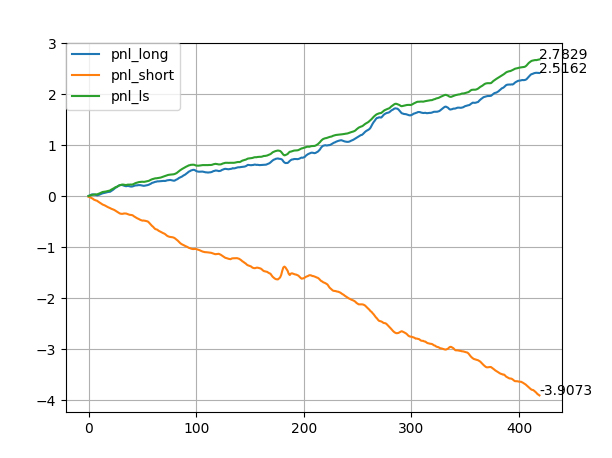
\includegraphics[width=0.8\textwidth]{2.PNG}
\end{center}
\caption{CNN1d pnl fugure}
\label{FIG.1}
\end{figure}

经过上面的研究,取得了不错的效果,但是效果还不够。因此又做了大量尝试,结果都差不多。直接想到应该继续加深模型,有了以下这些模型结果

~\\
模型12:普通CNN1d((CNN1d(5,1)+batchnorm)*3+relu+CNN1d(3,1)+

dropout+batchnorm+relu+

CNN1d(3,1)+CNN1d(3,1)+CNN1d(3,1)+batchnorm+relu+avg+dropout+

CNN1d(3,1)+CNN1d(3,1)+CNN1d(3,1)+batchnorm+relu+avg+dropout+

CNN1d(3,1)+CNN1d(3,1)+CNN1d(3,1)+batchnorm+dropout+avg+avg+linear)

模型深度提高,效果提高,骨架结构还是采用的之前研究的结构,兼顾稳定性和效果。

模型表现{\kaishu \small IC: 0.072, pnl:2.821}

~\\
模型13:普通CNN1d((CNN1d(5,1)+batchnorm)*3+relu+CNN1d(3,1)+

dropout+batchnorm+relu+

CNN1d(3,1)+CNN1d(3,1)+CNN1d(3,1)+batchnorm+relu+avg+dropout+

CNN1d(1,1)+CNN1d(1,1)+CNN1d(1,1)+batchnorm+dropout+avg+avg+linear)

不妨想到,cnn的格式可以不拘于一格,也体现出跨步跳跃的情况。不妨采用kernel\_size = 1的卷积层作为最后三层,经过大量实验,效果超过了同层的三卷积层。从理解上,应该是类似\par bottleneck结构。在高维卷积后面加入1维卷积效果会有提升。

模型表现{\kaishu \small IC: 0.075, pnl:2.830}

~\\
模型14:普通CNN1d((CNN1d(5,1)+batchnorm)*3+relu+CNN1d(3,1)+

dropout+batchnorm+relu+

CNN1d(3,1)+CNN1d(3,1)+CNN1d(3,1)+batchnorm+relu+avg+dropout+

CNN1d(1,1)+relu+CNN1d(1,1)+relu+CNN1d(1,1)+batchnorm+dropout+avg+avg+linear)

继续跳跃,在每个1卷积层后加入relu.

模型表现{\kaishu \small IC: 0.074, pnl:2.789}

~\\
模型15:普通CNN1d((CNN1d(5,1)+batchnorm)*3+relu+CNN1d(3,1)+

dropout+batchnorm+relu+

CNN1d(3,1)+CNN1d(3,1)+CNN1d(3,1)+batchnorm+relu+avg+dropout+

CNN1d(3,1)+CNN1d(3,1)+CNN1d(3,1)+batchnorm+relu+avg+dropout+

CNN1d(1,1)+relu+CNN1d(1,1)+relu+CNN1d(1,1)+batchnorm+dropout+avg+avg+linear)

模型深度继续增加,发现效果变差。经过实验,CNN的层数不适合超过9层,因此,对于\par CNN1d的模型首先必须要确定模型能承受的CNN层数上限。对于以后的模型设计有很大帮助。

模型表现{\kaishu \small IC: 0.055, pnl:2.520}

~\\
模型15:普通CNN1d((CNN1d(5,1)+batchnorm)*3+relu+CNN1d(3,1)+

dropout+batchnorm+relu+

CNN1d(1,1)+CNN1d(3,1)+batchnorm+relu+avg+dropout+

CNN1d(1,1)+relu+CNN1d(1,1)+relu+CNN1d(1,1)+batchnorm+dropout+avg+avg+linear)

模型结构进行大的修改,发现还有实验的新天地。也就是不同kernel\_size的组合。经过之前模型的实验已经知道,尽可能多种类的kernel\_size的效果更好,但是稳定度较差。那么思路应该是尽可能尝试不同的kernel\_size的组合。对于稳定性,采用其他层加以巩固。

模型表现{\kaishu \small IC: 0.065, pnl:2.758}

表现如下:
\begin{figure}[H]

\begin{center}
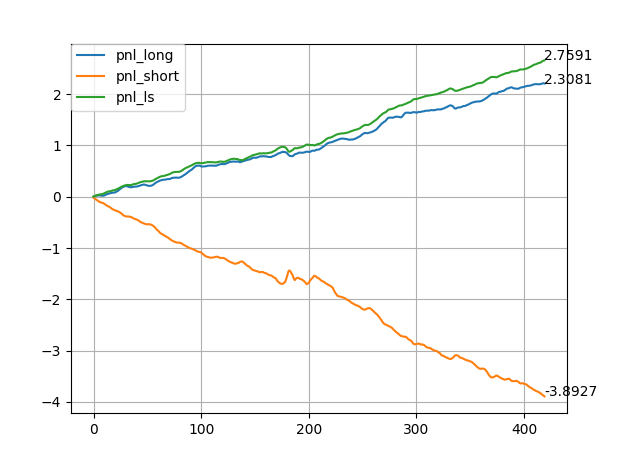
\includegraphics[width=0.8\textwidth]{1.PNG}
\end{center}
\caption{CNN1d pnl fugure}
\label{FIG.2}
\end{figure}

\subsection{改进思路}
\begin{itemize}
  \item [0)]
    这一周在CNN1d上做了大量实验。也找到了做实验的办法。找到了一些好的模型,获得了大量认知,也明白了传统backbone搭建的思路,为什么要这么做,自己可以用这些认知自己搭建模型,而不是复现原先有的模型。
  \item [1)]
    其中过一个改进思路是CNN的提取。比如stride,dilation,groups等参数,在这个场景下如何细致的影响CRNN的最后结果。这些细致的改变最后造成的影响是非常大的。比如可以采用之前研究的多种dilation叠加的办法,多种stride叠加的办法,增强cNN的感受野。
  \item [2)]
    另一个思路是kernel\_size的不同组合。提高表现,同时,在表现好的模型上运用稳定性模块,防过拟合模块,resnet,shortcut等内容.
\end{itemize}


\section{第二、CNN2d}
\subsection{综述}
对于CNN1d有了大量启发,忍不住尝试了CNN2d的结果,在原有结果上进行实验和更改。结论是CNN2d不适合这个任务,不管怎么改,模型跑的又慢又占显存,效果还不好。稳定性也不好。下面把思路和实验结果列出。

\subsection{convGRU}
模型1:CNN2d(CNN2d*2+CNN2d+avgpool+linear+dropout+relu)

{\kaishu \small IC: 0.041, pnl:2.2}


~\\
模型2:CNN2d(CNN2d*2+batchnorm+relu+CNN2d*2+batchnorm+

avgpool+linear+dropout+relu)

{\kaishu \small IC: 0.043, pnl:2.3}

~\\
模型3:CNN2d(CNN2d+batchnorm+relu+CNN2d+batchnorm+

CNN2d+batchnorm+relu+CNN2d+batchnorm+

avgpool+linear+dropout+relu)

{\kaishu \small IC: 0.039, pnl:1.9}

~\\
模型4:CNN2d(CNN2d*2+batchnorm+relu+CNN2d+batchnorm+

CNN2d*2+batchnorm+relu+CNN2d+batchnorm+

avgpool+linear+dropout+relu)

由此可见,模型深度提高,模型效果变差,CNN2d的深度上限不能超过5,同时稳定迅速下降。不适合再次深入

{\kaishu \small IC: 0.037, pnl:2.1}

~\\
模型6:CNN2d(CNN2d*2+relu+batchnorm+CNN2d*2+relu+batchnorm+

CNN2d*2+relu+batchnorm+dropout+avgpool+linear+dropout+relu)

{\kaishu \small IC: 0.041, pnl:2.3}

~\\
模型7:CNN2d(CNN2d*2+batchnorm+avgpool+CNN2d*2+batchnorm+avgpool+

CNN2d*2+batchnorm+avgpool+linear+dropout+relu)

在附近进行了大量尝试,效果都差不多,稳定性也不好

{\kaishu \small IC: 0.043, pnl:2.2}

~\\
模型8:CNN2d(CNN2d*2+relu+batchnorm+avgpool+CNN2d*2+relu+batchnorm+

avgpool+CNN2d*2+relu+batchnorm+avgpool+

dropout+avgpool+linear+dropout+relu)

不管怎么改变,模型IC和pnl始终在较低水准附近徘徊,CNN2d本身限制也很多,不适合做很多数据处理,跳跃的结构也很有限。

{\kaishu \small IC: 0.041, pnl:2.3}


\subsection{改进思路}
\begin{itemize}
  \item [0)]
    CNN2d不适合这个这个任务..

\end{itemize}

\section{第四、总结}
\begin{itemize}
  \item [1)]
  这一周,时间比较紧张,主要是进行了大量实验,自己研究出一批CNN1d模型,同时会在这些模型上深入。从dialtion,groups,stride上下功夫,同时在不同kernel\_size的组合上下功夫。
  \item [2)]
  第二,对于模型稳定性,除了初始化条件和激活函数的办法,这个办法,还有数据预处理,梯度改善等。最主要的办法还是从模型上下手。以后定下来最后加一层softmax,同时初始化条件采用xvier\_norm初始化函数
  \item [3)]
  第三,对于CNN1d系列,下周就继续搭建自己的backbone。尝试avg的不同位置,relu的不同位置,加入batchnorm,利用已经积累的CRNN调整的经验进行搭建。同时如果发现附近的结果表现提高都有限。就进行跳跃。迈一大步看看别的情况。
\end{itemize}


\end{document} 